To evaluate the optimization result, we benchmark the implementation on a 64 bit Arch Linux machine with a 3GHz Intel Skylake CPU of i7-6600U. The 64 bit multiplication (mul, mulx) is 1 op/cycle, and 64 bit addition with carry (adc, adcx, adox) is 1 op/cycle. The peak performance is therefore 2 ops/cycle (6 Gops/s) on 1 core. GCC 6.1.1 is used with compile flags -O3 -mavx2 -mbmi2 -madx. 

Based on the recommended Elliptic curve parameters from the guidance standard \cite{Brown:2010}, we have chosen five predefined curves with various key sizes: 192, 224, 256, 384, 521 bits. All versions of implementation have been validated by using Google Unit test, by checking the ECDH key exchange result. In the end we compare our implementation with OpenSSL, the well known open source library to check our implementation effect. We linked our program to a locally compiled version of OpenSSL . 

\begin{figure}[h!]\centering
  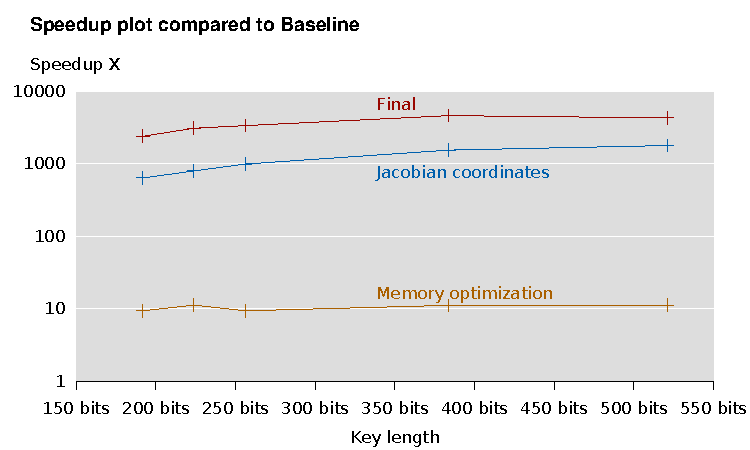
\includegraphics[scale=0.7]{speedup}
  \caption{Speedup plot compared to Baseline \label{speedup}}
\end{figure}
\begin{figure}[h!]\centering
  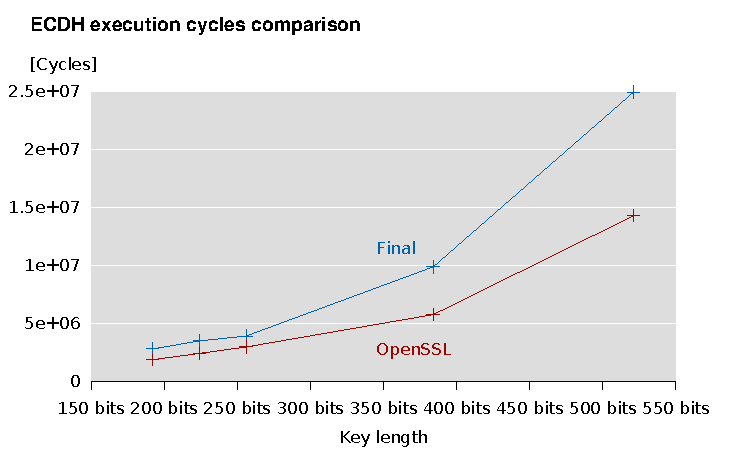
\includegraphics[scale=0.7]{ecdh}
  \caption{ECDH execution cycles comparison\label{ecdh}}
\end{figure}
\begin{figure}[h!]\centering
  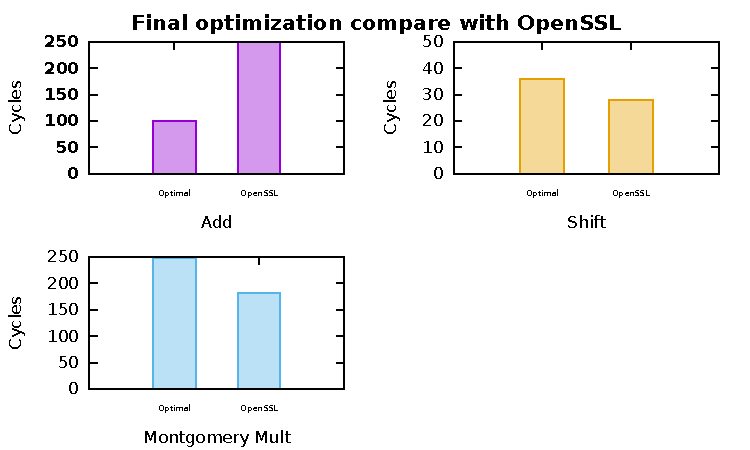
\includegraphics[scale=0.5]{openssl}
  \caption{Final optimization compared with OpenSSL\label{openssl}}
\end{figure}

In the speedup comparison(Fig.~\ref{speedup}) three crucial numbers are shown. It can be clearly seen that the Final implementation can execute the key exchange process 5000 times(TO BE CHANGED) faster than the baseline in almost all the key lengths. The first milestone of memory optimization gives us about 10 times speedup, whereas Jacobian coordinates version of code can run 1000 times(TO BE CHANGED) faster. This is due to the fact that the algorithm thus the operation count has changed fundamentally after we applied the projective coordinates and precomputed the Elliptic curve points in order to save unnecessary operations. The speedup result is satisfactory and reasonable as the first two versions of implementations contain costly memory allocations and expensive computation that can be avoided. The real performance boost is between the Final version and Jacobian coordinates, after applying the CPU based optimizations mentioned in previous section 3. It can be seen that it give us another 5x(TO BE CHANGED) speedup, showing the efficiency of the final implementation.

Next we run the same operation with OpenSSL library and compare the computation cycles. It is no surprise that with the increasing of the key length the required cycles also increase rapidly(Fig.~\ref{ecdh}). Our number of required cycles remains the save level with OpenSSL, in key length range of less than 256 bits, yet falls behind OpenSSL with larger key length. Individual operations of integers are the main component of our algorithm. To see how good is our implementation we choose Montgomery multiplication to compare with OpenSSL(Fig.~\ref{openssl}).This comparison is done with the same random large integers for both Final implementation and OpenSSL. Our implementation runs slightly behind OpenSSL. 

\begin{figure}[h!]\centering
  \includegraphics[scale=0.7]{perfplot1}
  \caption{Performance plot of baseline and memory optimization\label{perfplot1}}
\end{figure}
\begin{figure}[h!]\centering
  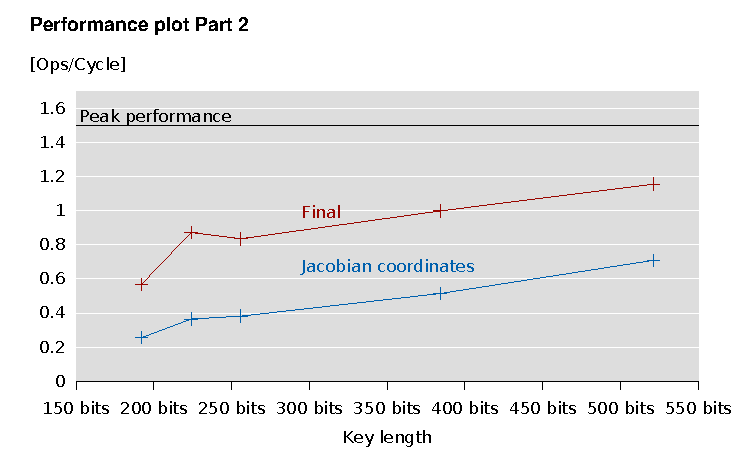
\includegraphics[scale=0.7]{perfplot2}
  \caption{Performance plot of Final optimization and Jacobian coordinates\label{perfplot2}}
\end{figure}

Performance plots (Fig.~\ref{perfplot1} and Fig.~\ref{perfplot2}) reflect if the implementation can make full use of the machines' computation ability. In Fig.~\ref{perfplot1} the first comparison is done by showing the effect of memory optimization. It is clear that with large amount of memory allocation, the baseline performance is really limited. In Fig.~\ref{perfplot2} we begin to see the real performance boost that comes from later optimization. Between these two figures the operation counts change drastically, thus we separate the performance plots. The peak performance here is calculated by considering the ratio of additions and multiplications. With 1 add and 1 mult per cycle and two times of add out of one mult (2 add : 1 mult), we can draw the line of peak performance at 1.5 ops/cycle. As we can see the final optimization are close to the peak performance with large key size. The highest performance of the final implementation arrives when the key length of 521 bits, with 1.15/1.5 = 77\% (TO BE CHANGED) of the peak performance. In all cases the performance increases as the key size grows. It can be explained that with relatively shorter the key size, the warm up process would dominate the calculation loop thus the constant overlap can prevent the program from running through the loop to reach the peak performance. Whereas with larger key length the loop takes most of the computation and the peak performance will happen within the loop.

\begin{figure}[h!]\centering
  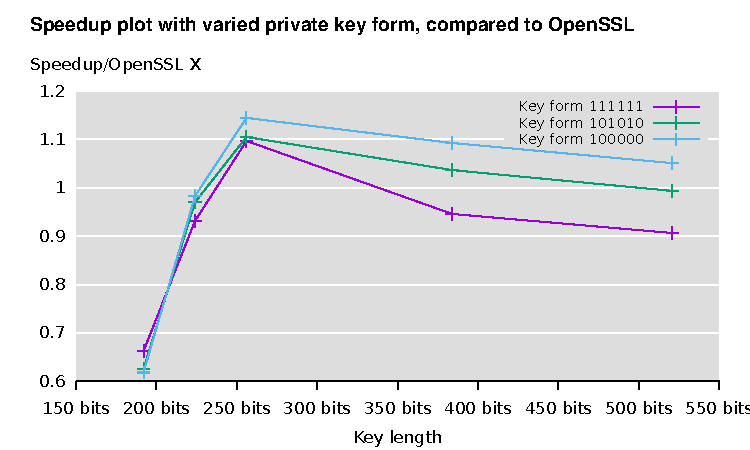
\includegraphics[scale=0.7]{keysize}
  \caption{Speedup plot with varied private key form, compared to OpenSSL\label{keysize}}
\end{figure}

Fig.~\ref{keysize} gives us another perspective of how different key forms could influence the speedup.  In all the simplified private key form that consist of only zeros and ones, our speed of processing EDCH is faster than OpenSSL. The key forms that consist only ones has the worst performance since it requires redundant integer operations that are unavoidable. It is an interesting future work that would allow us to optimize the algorithm based on the combinations of varied key forms. 